\documentclass[parskip=full,11pt]{scrartcl}
%\usepackage{pdfpages}
\usepackage[utf8]{inputenc}
\usepackage[T1]{fontenc}
\usepackage[german]{babel}
\usepackage[yyyymmdd]{datetime} 
\usepackage{hyperref}
\usepackage[toc, nonumberlist]{glossaries}
\usepackage{csquotes}
\usepackage{graphicx}
\hypersetup{
 		pdftitle={Entwurf},
 		bookmarks=true,
 }
\usepackage{fancyhdr}%<-------------to control headers and footers
\usepackage[a4paper,margin=1in,footskip=.25in]{geometry}
\fancyhf{}
\fancyfoot[C]{\thepage} %<----to get page number below text
\pagestyle{fancy} %<-------the page style itself
 
\title{Entwurf}
\subtitle{Autorisierungsmanagement für eine virtuelle Forschungsumgebung für Geodaten}
\author{Alex\\Anastasia\\Atanas\\Dannie\\ Houra\\Sonya\\}
\date{11.01.18}
 % define custom lists
\usepackage{enumitem}



\usepackage{linegoal,listings}
\newsavebox{\mylisting}
\makeatletter
\newcommand{\lstInline}[2][,]{%
	\begingroup%
	\lstset{#1}% Set any keys locally
	\begin{lrbox}{\mylisting}\lstinline!#2!\end{lrbox}% Store listing in \mylisting
	\setlength{\@tempdima}{\linegoal}% Space left on line.
	\ifdim\wd\mylisting>\@tempdima\hfill\\\fi% Insert line break
	\lstinline!#2!% Reset listing
	\endgroup%
}
\makeatother
\setlength{\parindent}{0pt}% Just for this example

\lstset{basicstyle=\footnotesize\ttfamily,breaklines=true}
\lstset{framextopmargin=50pt,frame=bottomline,showstringspaces=false,upquote=true}


\RedeclareSectionCommand[style=section,indent=0pt,font=\usekomafont{partnumber}]{part}
\renewcommand*{\partformat}{\thepart\enskip}

\RedeclareSectionCommand[beforeskip=0pt ,afterskip=0pt]{subparagraph}



\newcommand{\class}[1]{\subsubsection*{\lstinline[basicstyle=\ttfamily\large]{#1}}}

% command for an attribute
\newcommand{\atr}[4]{\lstinline{[#3]} \textbf{\lstinline{#1 : #2}} \newline #4}

% command for a method
\newcommand{\mtd}[5]{\lstinline{[#4]} \textbf{\lstinline{#1(#3) : #2}} \newline #5}

% command for a constructor
\newcommand{\ctr}[4]{\lstinline{[#3]} \textbf{\lstinline{#1(#2)}} \newline #4}
%command for formating an inline source code
\newcommand{\inlinecode}[1]{\lstInline[breaklines=true]{#1}}

% make the bullet symbol in lists a circle for level 2
\renewcommand{\labelitemii}{$\circ$}




 
\begin{document}
 
 \begin{titlepage}
 	
 	\begin{center}
 	
\includegraphics[width=0.5\linewidth]{res/KITLogo.png}\\
 	\vspace{2cm}
 	{\scshape\LARGE\bfseries Entwurf \par}
 	\vspace{0.5cm}
 	{\scshape\Large Praxis der Softwareentwicklung\\}
 	\vspace{1cm}
 	{\scshape\Large Wintersemester 17/18\\}
 	\vspace{2cm}
 	{\huge\bfseries Autorisierungsmanagement für eine virtuelle Forschungsumgebung für Geodaten\par}
 	\vspace{2cm}
 	\vfill
 	{\bfseries {\Large Autoren}:\par}
 	{\Large Bachvarov, Aleksandar }\\
 	{\Large Dimitrov, Atanas }\\
 	{\Large Mortazavi Moshkenan, Houraalsadat }\\
 	{\Large Sakly, Khalil }\\
 	{\Large Slobodyanik, Anastasia }\\
 	{\Large Voneva, Sonya}\\
 	\vfill
 	{\large 11.01.18 \par}
 	\end{center}
 \end{titlepage}
 
 \tableofcontents
 
 \newpage
 \section{Einleitung}
 
 Während der Entwurfsphase wurde das Konzept für das zu erstellende Produkt formuliert. Die in diesem Dokument definierte Softwarearchitektur legt die Struktur und das Verhalten des Produkts fest. Durch Bestimmung grundlegender Entwurfsentscheidungen haben sich einige sinnvolle Änderungen zum Pflichtenheft ergeben. \\
Für die Funktion „Benutzer suchen“ wurden Suchparameter erweitert: die Suche soll anhand von Name, Email sowie Domain des Benutzers möglich sein. 
Nach dem Löschen einer Ressource werden alle Benutzer, die Besitzerrechte für diese Ressource hatten, benachrichtigt. 
Als Ressourcendaten werden auch Typ und kurze Beschreibung der Ressourcen gespeichert. 
Administratoren des Portals sollen in der Lage sein andere Benutzer zu blockieren.

 
 \section{Architektur}
 
 \subsection{Model View Template (MVT)} 
 	
 	
 \begin{figure}[ht!]
 \centering
 \begin{flushleft}
 Beim Design des Autorisierungsmanagement Web-Portal wird schnell deutlich, dass eine strikte Trennung
zwischen Datenbank, Applikationslogik (Code) und Benutzeroberfläche (view) von Vorteil ist. Das Model-View-Template-Prinzip (MVT) realisiert diese Trennung und wird in der Webanwendung eingesetzt.\\
 \end{flushleft}
  	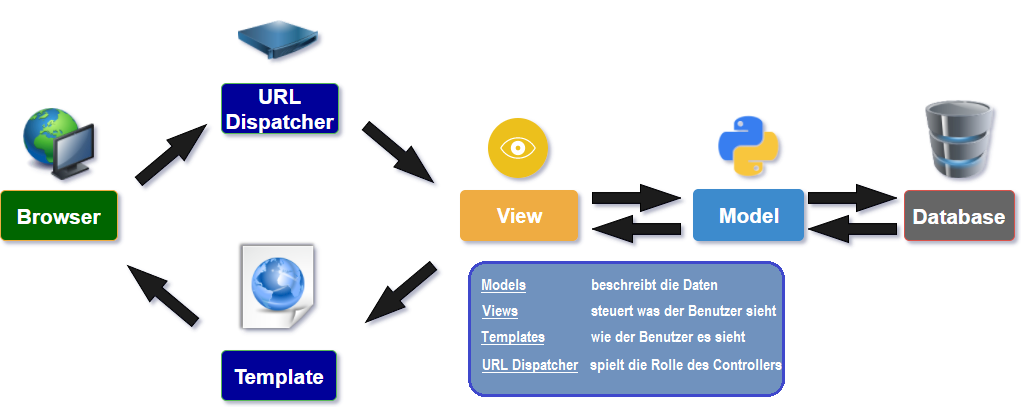
\includegraphics[width=18cm, height=12cm]{res/MVTdiagramm.png}\\
  	    \caption{MVT Architektur}
 	\vspace{2cm}
 	\end{figure}
 	 \newpage

 	\begin{flushleft}
 	\textbf{A-} Der \textbf{URL-Dispatcher} \emph{(urls.py)} ordnet die angeforderte URL einer \textbf{View-Funktion} zu und ruft sie auf.\\
 	\textbf{B-} Die \textbf{View-Funktion} \emph{(views.py)} führt die angeforderte Aktion aus, bei der normalerweise in die Datenbank gelesen oder geschrieben wird. es kann auch andere Aufgaben beinhalten.\\
 	\textbf{C-} Das \textbf{Model} \emph{(models.py)} definiert die Daten in Python und interagiert damit. Dies ist normalerweise in einer relationalen Datenbank \emph{(SQLite)} enthalten.\\
 	\textbf{D-} Nach der Ausführung der angeforderten Aufgaben gibt die \textbf{View} ein HTTP-Antwortobjekt an den Webbrowser zurück, normalerweise nach dem Übergeben der Daten durch ein \textbf{Template}.\\
 	\textbf{E-} \textbf{Template} gibt normalerweise HTML-Seiten zurück. Die Django-Template-sprache bietet HTML-Autoren eine einfach zu erlernende Syntax und bietet gleichzeitig die gesamte für die Präsentationslogik erforderliche Leistung. \\
 	\end{flushleft}


 	


 \subsection{Paketstruktur}%oder Paketen?
 
 \subsection{Entwurfsmuster}
 
  \subsection{URL Verzeichnis}
Alle Interaktionen zwischen den Benutzern und dem Produkt werden durch eine graphische Benutzeroberfläche (GUI) unterstützt. GUI des Produkts wird als eine Webseite dargestellt, wobei sämtlicher Inhalt und Funktionalität unter URL Verzeichnis abgelegt werden (Abbildung). %TODO bild
\textbf{pse-authoritation.com} – Mockup-Seite, dient zum Einloggen in das Portal, enthält Autorisierungsformular und wird nach der Entwicklung durch Autorisierungsmanagement des Systems, in welches das Projekt integriert wird, ersetzt. 
 
\renewcommand{\labelitemi}{$\bullet$}
\renewcommand{\labelitemii}{$\bullet$}
\renewcommand{\labelitemiii}{$\bullet$}
\begin{itemize}[itemsep=0pt]
\item \textbf{{\textbackslash}profil} - Benutzerprofil-Seite, enthält persönliche Information des Benutzers und Übersicht der Requeste, die an den Benutzer adressiert sind.
Benutzerprofil-Seite ist mit Subseiten versehen:
\begin{itemize}[itemsep=0pt]
\item \textbf{{\textbackslash}handle{\_}request{\_}$<$requestID$>${\_}$<$userID$>$} - Dialog für Bearbeitung des Requests, enthält ``Annehmen''- und ``Ablehnen``-Buttons, sowie ein Eingabefeld für kurze Begründung.
\item \textbf{{\textbackslash}edit{\_}name} - Dialog mit Eingabefeld für Editieren des Namens des Benutzers, wird nach dem Klicken des ``Ändern``-Buttons sichtbar.
\item \textbf{{\textbackslash}resources} - Seite mit Übersicht von Ressourcen, für die der Benutzer Besitzerrechte hat. Diese Seite enthält Subseiten:
\begin{itemize}[itemsep=0pt]
\item \textbf{{\textbackslash}add{\_}new{\_}resource} - Seite für Erstellen neuer Ressourcen. Enthält Upload-Dialog, Dialog für Vergabe von Rechten und Eingabefelder für Namen und Beschreibung der Ressourcen.
\item \textbf{{\textbackslash}$<$resourceID$>${\_}edit{\_}permissions} - Seite für Vergabe und Entzug von Rechten für die Ressource.
\item \textbf{{\textbackslash}$<$resourceID$>${\_}send{\_}deletion{\_}request{\_}} - Dialog für Absenden von Löschrequest für die Ressource.
\end{itemize}
\end{itemize}
\item \textbf{{\textbackslash}manage{\_}users} - Administratorseite für Benutzerverwaltung, enthält Liste von Benutzern und Subseiten:
\begin{itemize}[itemsep=0pt]
\item \textbf{{\textbackslash}block{\_}user} - Dialog zum Blockieren des Users.
\item \textbf{{\textbackslash}delete{\_}user} - Dialog zum Löschen des Users.
\item \textbf{{\textbackslash}edit{\_}permissions} - Dialog zur Änderung von Rechten des Benutzers.
\end{itemize}
\item \textbf{{\textbackslash}manage{\_}resources} - Administratorseite für Ressourcenverwaltung, enthält Liste von Ressourcen und Subseiten:
\begin{itemize}[itemsep=0pt]
\item \textbf{{\textbackslash}edit{\_}permissions} - Dialog zur Änderung von Zugriffsrechten für die Ressource. 
\item \textbf{{\textbackslash}delete{\_}resource} - Dialog zum Löschen der Ressource.
\end{itemize}
\item \textbf{{\textbackslash}resources{\_}owerview} - Übersicht von Ressourcen, enthält Liste aller Ressourcen und folgende Subseiten:
\begin{itemize}[itemsep=0pt]
\item \textbf{{\textbackslash}$<$resourceID$>${\_}info} - enthält Metadaten der Ressource.
\item \textbf{{\textbackslash}$<$resourceID$>${\_}send{\_}request} - Dialog zum Absenden des Requests für die Ressource.
\end{itemize}
\item \textbf{{\textbackslash}<resourceID>} - Ressourcenseite, enthält Metadaten und Link für Zugriff auf die Ressource.
\end{itemize} 

 
 
 \section{Datenhaltung}
 
 Die Benutzer des Web-Portals, ihre Ressourcen und die von ihnen gesendeten Requests werden als Tabellen in einer Datenbank gespeichert. Als Syntax wird SQLite3 verwendet.
 \subsection{Datenbank}
 \begin{figure}[ht!]
 	\centering
 	\includegraphics[width=0.75\textwidth]{res/database.png}
 	\caption{Datenbankschema}
 \end{figure}
 \newpage
 Die Tabelle ``Benutzer`` speichert einen eindeutigen Identifikator des Benutzers, seinen Vor- und Nachnamen, sowie das Datum, an dem er sich registriert hat. Zusätzlich hat die Tabelle eine Spalte ``ist\char`_admin``, die zur Unterscheidung zwischen ``normalem`` Benutzer und Administrator dient.\\ Tabelle ``Request`` hat folgende Spalten: einen eindeutigen Identifikator, Erstellungsdatum, Typ des Requests (Zugriffs- oder Löschrequest), Identifikator der Ressource, für die der Request gesendet wird, und Identifikator des Absenders. \\
 Tabelle ``Resource`` speichert einen eindeutigen Identifikator zu jeder Ressource, ihren Namen, Typ, kurze Beschreibung und Erstellungsdatum.\\
 Tabelle ``Permission`` beinhaltet Einträge der Form: Benutzer-Ressource-Rechte (Zugriffs- oder Besitzerrechte). \\
 Die Funktion der Tabelle ``ReceivedRequest`` ist die gesendeten Requests, ihre Empfänger, sowie ihren Typ zu speichern. Darum hat sie als Spalten Identifikator eines Benutzers und eines Requests und einen Typ des Requests
 
 \subsection{Logging}
 Mithilfe von einem externen Django Module (``Logging``) wird eine Log-Datei geführt. Diese Datei beinhaltet zeitlichgeordnete Ereignisse vom System. Informationen wie Senden eines Requests, Bearbeitung eines Requests, Erstellen/Löschen einer Ressource und Editieren von Rechten können der Log-Datei entnommen werden. Zu jedem Ereignis wird auch den genauen Zeitpunkt gespeichert.
 
 
 \section{Paketenübersicht}
 
 
 \section{Klassenübersicht}
 
  \paragraph*{Klasse Owner}
 \class{Owner extends User}
 bla bla
 
 \subparagraph*{Konstruktoren} % skip this if there are no constructors
\begin{itemize}
	\item \ctr{User}{a:String}{public}{
	bla
	}
\end{itemize}
\paragraph*{Attribute} % skip this if there are no attribute
\begin{itemize}
	\item \atr{name}{String}{private}{
	bla 
	}
\end{itemize}
\subparagraph*{Methoden}  % skip this if there are no methods
\begin{itemize}
	\item \mtd{foo}{String}{a:String}{public}{
	bla  \inlinecode{USER_ID}
	}
\end{itemize}
 
 \section{Sonstige Diagrammen}
 \subsection{Zugriffsrequest schicken}
 \begin{figure}[ht!]
 	\centering
 	\includegraphics[width=\textwidth]{res/sendAccessRequest.png}
 	\caption{Zugriggsrequest schicken}
 	\label{fig:sendAccReq}
 \end{figure}
 
Von irgeneiner Viewklasse wird die Methode \enquote{sendAccessRequest(resourceID )} auf dem Benutzer \enquote{a}  aufgerufen. Erstens wird eine AccesRequest Instanz \enquote{b} erstellt und in der Datenbank gespeichert. Danach wird die Ressource, für den das Request geschickt wurde, von der Datenbank geholt und in der Variable \enquote{r} gespeichert. Auf der Ressourceninstanz \enquote{r} wird dann getOwners() aufgerufen, was alle Besitzer des Ressource liefert. Auf allen Instanzen von diesen Besitzer(auf dem Diagramm als die Variable \enquote{list} bezeichnet) wird die Methode  \enquote{addAccessRequest(request)} aufgerufen. Das fügt den Request in der Liste der bekommenen, aber noch nicht bearbeiteten Requesten, hinzu. Eine passende Lognachricht (die in dem Diagramm gegebene ist nur als Beispiel gegeben, die echte Nachricht wird anders sein) wird in der Logdatei durch die Methode \enquote{info()} gespeichert. Danach wird eine Instanz der Djangoklasse \enquote{Emailmessage} erstellt. Als Parameter ist die Variable \enquote{list} gegeben. Damit ist gemeint, dass die Klasse alle Emails von den Besitzern in List nimmt. Der Konstruktor der Klasse nimmt auch andere Parameter als Emailnachricht, Sender usw, die im Diagramm nicht bezeichnet sind. Nach dem erfolgreichten Schicken der Emails mit der Methode  \enquote{send()} wird eine Lognachricht dafür in der Logdatei gespeichert. 
 
  \newpage
 \subsection{Zugriffsrequest genehmigen}
 \begin{figure}[ht!]
 	\centering
 	\includegraphics[width=\textwidth]{res/allowAccessPermission.png}
 	\caption{Zugriffsrequest genehmigen}
 \end{figure}
 
 Von irgeneiner Viewklasse wird die Methode \enquote{sendAccessRequest(resourceID )} auf dem Besitzer \enquote{a}  aufgerufen. Danach wird der Request von der Datenbank geholt in in der Variable \enquote{req} gespeichert. Danach wird auf \enquote{req} getSender aufgerufen und das Ergebnis(der Benutzer, der das Request geschickt hat) wird dann in \enquote{u} gespeichet. Das Gleiche passiert für das durch den Request angefragte Ressource durch die Methode \enquote{getResource()}. Auf \enquote{u} wird dann \enquote{addAccessPermission(resource)} aufgerufen, was intern der Benutzer \enquote{u} in der Liste \enquote{accessPermission} von Ressource hinzufügt. Eine Lognachricht wird in der Logdatei gespeichert. Die Methode \enquote{delete(requestID)} löscht den Request von der Datenbank. Von hier an ist das Diegramm ähnlich bis gleich zum Ende des Diegramms \hyperref[fig:sendAccReq]{Zugriffsrequest schicken}. 
 
 \newpage
	
 \end{document}
 \grid
